\documentclass[a4paper]{report}
\usepackage{amsmath}
\usepackage{blindtext}
\usepackage{blindtext}
\usepackage[utf8]{inputenc}
\usepackage{graphicx}
\usepackage{appendix}


%for MATLAB code:
\usepackage{listings}

\usepackage{geometry}
\geometry{a4paper, margin=1in}


\begin{document}
\title{\Huge Finite Elements}
\author{Rick Koster \\ Ruben Termaat}
\date{\today}
	
\maketitle

\tableofcontents


\chapter{1D-case}



On the 1D interval of $x = [0,1]  $, we consider a steady-state convection-diffusion-reaction equation, with homogeneous Neumann boundary conditions. The following equations apply to this domain:

\begin{equation}
\begin{cases} 
-D\triangle u + \lambda u = f(x),\\ -D\frac{du}{dx}(0) = 0 ,\\ -D\frac{du}{dx}(1) = 0
\end{cases} 
\end{equation}
\bigskip

Here $ \triangle$ equals the $\nabla \cdot \nabla$ operator. The function f(x) is a given funtion, where D and $\nabla$ are positive real constants. In order to solve this boundary value problem (BVP), first the interval is divided in n-1 elements(n = positive integer). This results in the domain being divided in elements: $e_i = [x_i, x_{i-1}]$ where $i={1,2,..,n}$. 

In order to solve this BVP, the solutions for the given equations will first be calculated and then computed using MATLAB codes.


\section{Boundary value problem 1D}
\vspace{5mm}

In order to find the Weakform of the given equations of (1.1), we first multiply both sides by $\phi$ and integrate both sides over the domain $\omega$.


\begin{equation}
	 \int_{\Omega} \phi(-D\triangle u + \lambda u )d\Omega = \int_{\Omega} \phi f(x) d\Omega 
\end{equation}	
\smallskip

Now by rewriting and then using partial integration the following equation can be found:


\begin{equation}
	\int_{\Omega} (\nabla\cdot(-D\phi\nabla u) + D\nabla\phi\nabla u +\phi \lambda u) d\Omega = \int_{\Omega} \phi f(x) d\Omega 
\end{equation}
\smallskip

Applying Gauss on the first term on the left side of equation(1.3):


\begin{equation}
	\int_{\Omega}  \vec{n}\cdot(-D\phi \nabla u) d\tau + \int_{\Omega}  (D\nabla\phi\cdot\nabla u +\phi\lambda u )d\Omega = \int_{\Omega} \phi f(x) d\Omega 
\end{equation}
\smallskip

Using the boundary conditions from equations(1.1) the boundary integral equals to 0 and then the following weak formulation(WF) is found: \vspace{5mm}


(WF): \begin{equation}
\begin{cases} 
	$find u $\epsilon \sum =\{u$ $ smooth\}$ Such that:$ \\ \int_{\Omega}  (D\nabla\phi\cdot\nabla u +\phi\lambda u )d\Omega = \int_{\Omega} \phi f(x) d\Omega \\ \forall\phi $ $ \epsilon\sum 
\end{cases}\  
\end{equation}

\bigskip
The next step is to apply the Galerkin equations to the found diferential equation, where u is replaced by $ \sum_{j=1}^{n}c_i\phi_j $ and  $\phi(x)=\phi_i(x)$ with $i = [1,..,n]$. Filling this in equation (1.5) the following equation is found:

\begin{equation}
	\sum_{j=1}^{n}c_i\int_{0}^{1} (D\nabla\phi_i\cdot\nabla\phi_j +\lambda\phi_i\phi_j )d\Omega = \int_{0}^{1} \phi_i f(x) d\Omega
\end{equation}
\medskip

Which is of the form of $ S\vec{c} = \vec{f} $

\section{Element matrix}
Now the found Galerkin equations can be used to compute $ S_{ij}$  the element matrix, over a generic line element $ e_i$.

\begin{equation}
S\vec{c}=	\sum_{j=1}^{n}c_i\int_{0}^{1} (D\nabla\phi_i\cdot\nabla\phi_j +\lambda\phi_i\phi_j )d\Omega
\end{equation}
\medskip

Now to solve S we solve the following equation, over the internal line element.

\begin{equation}
S^{e_i}_{ij} = -D\int_{e_k}\nabla\phi_i\cdot\nabla\phi_j d\Omega+\lambda\int_{e_k}\phi_i\phi_j dx
\end{equation}


\section{Element vector}
Again using the found Galerkin Equations(1.6) in order to compute the element vector $f_i$ over a generic line-element.

\begin{equation}
f^{e_k}_i = \int_{e_k}\phi_i f dx
\end{equation}

\begin{equation}
	f^{e_k}_i =\frac{\lvert x_k-x_{k-1}\lvert}{(1+1+0)!}f(\vec{x}) =\frac{\lvert x_k-x_{k-1}\lvert}{2}
	\begin{bmatrix} f^{e_n}_{k-1}\\ f^{e_n}_{k}
	\end{bmatrix}
\end{equation}







\section{Boundary value problem 1D MATLAB routine}

\subsection{mesh and elmat code}
The first step in order to solve the BVP is to write a MATLAB routine that generates an equidistant distrubition of points over the given interval of $[0,1]$(generate a mesh with n-1 elements).

\begin{lstlisting}
	function [ x ] = GenerateMesh(int, N_elem)
	%GenerateMesh Creates a mesh for 1D problems
	
	
	% int = [0,1];
	% N_elem = 100;
	
	x = linspace(int(1,1),int(1,2),N_elem);
	
\end{lstlisting}
	
Using the codes to generate a mesh and the elmat, it is easier to use this 1D problem and adapt to a higher dimensional problem. The next step is to write a code that generates a two dimensional array, called the elmat.

\begin{lstlisting}
	function [ elmat ] = GenerateTopology( N_elem )
	%GenerateTopology Creates the topology for a 1D problem given mesh 'x'.
	
	% global N_elem
	elmat = zeros(N_elem,2);
	elmat(i,1) = i;
	elmat(i,2) = i + 1;

\end{lstlisting}

\subsection{Element matrix}

Now that the base MATLAB codes are made the element matrix and element vector codes can be written. The first step in this process is, is to compute the element matrix $S_{elem}$.

\begin{lstlisting}
	function [ Selem ] = GenerateElementMatrix( k, elmat, D, lambda, mesh)
	%GenerateElementMatrix Creates element matrix S_ek
	
	
	Selem = zeros(2,2);
	
	i = elmat(k,1);
	j = elmat(k,2);
	
	x1 = mesh(i);
	x2 = mesh(j);
	
	element_length = abs(x1-x2);
	
	slope = 1/element_length; 
	
	for m = 1:2
		for n = 1:2
			if m == n
				Selem(m,n) = element_length*((-1)^(abs(m-n))*D*slope^2
				+ (2)*lambda/6);
			else
				Selem(m,n) = element_length*((-1)^(abs(m-n))*D*slope^2
				+ (1)*lambda/6);
			end
			end
	
		end
	
	end
\end{lstlisting}

\bigskip

To generate a n-by-n matrix S, the sum over the connections of the vertices in each element matrix, over all elements has to be calculated. The following code computes this matrix.


\subsection{Assemble matrix S}

\begin{lstlisting}
	function [ S ] = AssembleMatrix( N_elem, int, lambda, D)
	% global N_elem 
	
	elmat = GenerateTopology(N_elem);
	
	S = zeros(N_elem,N_elem);
	
	for i = 1:N_elem-1
		Selem = GenerateElementMatrix(i, elmat, int, N_elem, D, lambda);
		for j = 1:2
			for k = 1:2
				S(elmat(i,j), elmat(i,k)) =
				S(elmat(i,j), elmat(i,k)) +	Selem(j,k);
			end
		end
	end


\end{lstlisting}



All the previous code will generate a large matrix S, from the element matrices $S_{elem}$ over each element.\\



\subsection{Element vector MATLAB routine}

The next step In order to solve the equation $S\vec{c}=F$ is to create a code to generate the element vector. This element vector provides information about note $i$ and node $i+1$, which are the vertices of element $e_i$.\\



\begin{lstlisting}
	function [ felem ] = GenerateElementVector( i, elmat, mesh )
	%GenerateElementVector Creates element vector f_ek
	
	
	felem = [0;0];
	
	k1 = elmat(i,1);
	k2 = elmat(i,2);
	
	x1 = mesh(k1);
	x2 = mesh(k2);
	
	element_length = abs(x1-x2);
	
	felem = (element_length/2*arrayfun(@functionBVP,[x1,x2]))';
	
	end
\end{lstlisting}

\smallskip

To generate the vector f, the sum over the connections of the vertices in each element matrix, over all elements $i\,\epsilon\, \{1,...,n-1\}$  has to be calculated. 

\bigskip

	
\begin{lstlisting}
	function [ f ] = AssembleVector( N_elem, int, lambda, D )
		
	f = zeros(N_elem,1);
	elmat = GenerateTopology(N_elem);
		
	for i = 1:N_elem-1
		felem = GenerateElementVector(i, elmat, int, N_elem);
		for j = 1:2
			f(elmat(i,j)) = f(elmat(i,j)) + felem(j);
		end
	end
\end{lstlisting}	




\subsection{Computing S and f}

Now if the previous matlab codes are run the following happens. Firstly a mesh and 1D topology is build, which is needed for the S matrix and f vector. The second step is to calculate the S matrix and f vector through the found equations of section 1.2 and 1.3. The final step is to use the found matrix and vector to solve the equation $Su=\vec{f}$.





\section{Main program}

The main program is simple written by assembling the previous created matlab code AssembleMatrix and AssembleVector and deviding the vector f by the matrix S.
\begin{lstlisting}
	function [ u ] = SolveBVP(  N_elem, int, lambda, D )
	
	S = AssembleMatrix( N_elem, int, lambda, D);
	f = AssembleVector( N_elem, int, lambda, D);
	
	%% Calculate u
	x = linspace(int(1),int(2),100);
	
	u = S\f;
	plot(x,u); 
	
	
\end{lstlisting}
The result of the plot is shown in figure(1.1).

\begin{figure}[ht!]
	\centering
	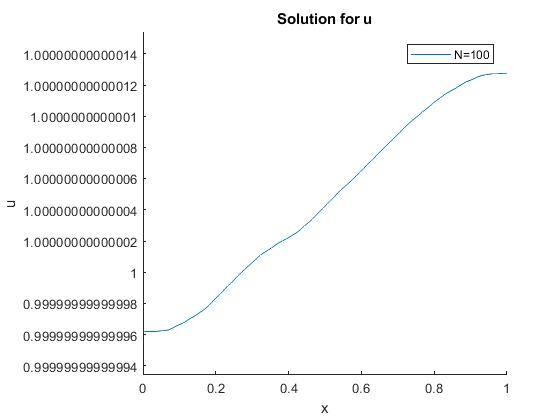
\includegraphics[width=150mm]{1Df1.jpg}
	\caption{showing the calculated u versus x, with N = 100,f(x)=1 \label{overflow}}
\end{figure}

\section{Solution for u}
The final step is to use the main program to solve $Su= \vec{f}$. Previously the S matrix and f vector were computed for $n = 100$. Now $u$ will be calculated for $f(x)=1$, $D=1$, $\nabla = 1$ and $N = 100$. The result of this is plotted in figure(1.2). 


\begin{figure}[ht!]
	\centering
	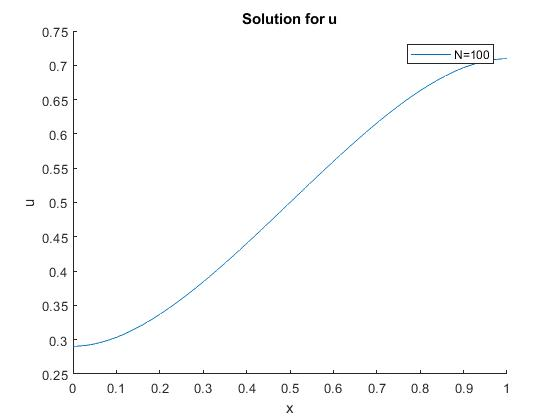
\includegraphics[width=150mm]{1Dfx.jpg}
	\caption{showing the calculated u versus x, with N = 100,f(x)=x 		 \label{overflow}}
\end{figure}



\vfill
\section{Experiment}

The next step is to see what happens when changing f(x) to $f(x)=sin(20x)$ and to see the difference for several values for n ($n=10,20,30,40,80,160)$ 

\vspace{5mm}
\begin{lstlisting}
	function [f] = functionBVP(x)
		f = sin(20*x);
	
		% f = x;
		%f = 1;
	
	end
	
	
	figure 
	hold on
	
	for N_elem = [10 20 40 80 100 160]
	mesh = GenerateMesh(int,N_elem);
	elmat = GenerateTopology(N_elem);
	S = AssembleMatrix( N_elem, lambda, D, mesh, elmat);
	f = AssembleVector( N_elem, mesh, elmat);
	
	x = linspace(int(1),int(2),N_elem);
	
	u = S\f;
	plot(x,u);
	
	legend('N=100')
	title('Solution for u')
	xlabel('x')
	ylabel('u')
	ax.box='on'
	end
	hold off
\end{lstlisting}

\newpage

Figure 1.3

\begin{figure}[ht!]
	\centering
	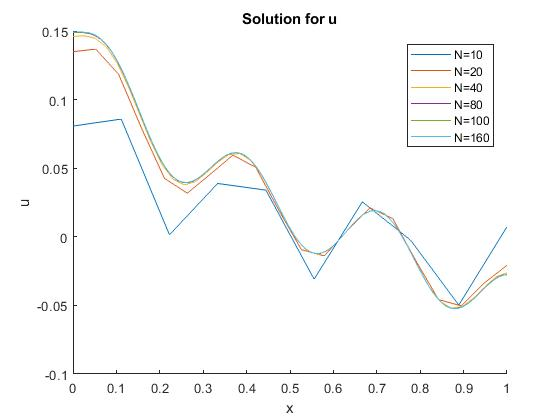
\includegraphics[width=150mm]{1Dfsinx.jpg}
	\caption{showing the calculated u versus x, with N =[10 20 40 80 ]100 160],f(x)=sin(x) \label{overflow}}
\end{figure}


\chapter{2D-case}


The obvious next step after solving a 1 dimensional boundary value problem BVP is to addept the 1D solutions and code to a 2 dimensional boundary value problem. To do this a real life problem is going to be used to solve. In 3rd world countries one of the big issues is the supply of fresh water. One way is to do this is to take square reservoirs, which is a porous medium, with several wells where water is extracted from the subsurface. The water pressure is equal to the hydrostatic pressure. As this is not on an infinite domain, mixed boundary conditions are used. These boundary conditions represent a model for the transfer of the water over the boundary to locations far away. To this extent, a square domain is considered with length 2 in meter: $\Omega= (-1; 1) x (-1; 1)$ with boundary $d\Omega$. Darcy's law for fluid determins the steady state equilibrium of this BVP, given by equation(2.1) :

\begin{equation}
\vec{v}=-\frac{k}{\mu}\nabla p
\end{equation}
\medskip

where p, k, $\mu$ and v, respectively denote the 
fluid pressure, permeability of the porous medium, viscosity of water and the fluid flow velocity. In this BVP the effect of gravity will not play a part as the problem is looked at in 2D. An accompanying assumption is incompressibility, so the extraction wells are treated as point sinks. This assumption can be made as the well its diameter is much smaller than the dimensions of the square reservoir. The extraction wells extract at the same rate in each direction, leading to the following boundary conditions(2.2).


\begin{equation}
	\nabla\cdot\vec{v}=-\sum_{p=1}^{n_{well}}Q_p\delta(x-x_p)=0,(x,y) \epsilon\Omega 
\end{equation}

where $Q_p$ denotes the water extraction rate by well k, which is located at $x_p$. Here $x$ equals $(x;y)$, the spatial coordinates.  We use the convention x = (x; y) to represent the spatial coordinates. The dirac Delta Distribution is characterized by equation(2.3).

\begin{equation}
	\begin{cases} 
		\delta(x) = 0,x \neq 0 \\ \int_{\Omega}\delta(x)d\Omega = 1,$  where $\Omega $  contains the origin.$
	\end{cases} 
\end{equation}

\medskip

For this BVP the following boundary condition is considered: 

\begin{equation}
	\vec{v}\cdot\vec{n}=K(p-p^H), \, (x,y)\, \epsilon\,  \partial\Omega
\end{equation}
\bigskip

Here $k$ denotes the transfer rate coefficient of the hormon between the boundary of the domain and its surroundings. The constant $p^H$ represents the hydrostatic pressure. In order to solve this BVP the values needed for all the constants are given in table (2.1).


\begin{table}[ht]
	\caption{Values of input parameters} % title of Table
	\centering % used for centering table
	\begin{tabular}{c c c} % centered columns (3 columns)
		\hline\hline %inserts double horizontal lines
		Symbol & Value & Unit\\ [0.5ex] % inserts table
		%heading
		\hline % inserts single horizontal line
		$Q_p$ & $50$ & $m^2/s$ \\ % inserting body of the table
		$k$ & $10^{-7}$ & $m^2$ \\
		$\mu$ & $1.002\cdot 10^{-3}$ & $Pa\cdot s$ \\
		$K$ & 10 & $m/s$ \\
		$p^H$ & $10^6$ & Pa \\ [1ex] % [1ex] adds vertical space
		\hline %inserts single line
	\end{tabular}
	\label{table:nonlin} % is used to refer this table in the text
\end{table}
\bigskip

In this BVP six wells are considered, which are located at:


\begin{equation}
	\begin{cases} 
		x_p=0.6\cos(\frac{2\pi (p-1)}{5}) \\ x_p=0.6\sin(\frac{2\pi (p-1)}{5})
	\end{cases} 
\end{equation}


\section{Boundary value problem 2D}
The first step to solving these equations using finite elements is to find to find the boundary value problem to solve. This is done by filling in equation(2.1) in both equation 2.2 and the boundary condition(2.4) in order to find the BVP in terms of p:
\vspace{5mm}

BVP:
\begin{equation}
	\begin{cases}
		-\frac{k}{\mu}\triangle\cdot\vec{p}=-\sum_{p=1}^{n_{well}}Q_p\delta(x-x_p)=0,\, \, (x,y) \, \epsilon \, \Omega\\
		-\frac{k}{\mu}\nabla\vec{p}\cdot\vec{n}=-\frac{k}{\mu}\frac{dp}{dn} =K(p-p^H), \, (x,y)\,  \epsilon  \, \partial\Omega
	\end{cases}
\end{equation}

\bigskip

The next step is to compute the weak formulation using the previous found BVP(2.6). By multiplying both sides by $phi(x)$ and integrating both sides over the domain $\Omega$ the weak formulation can be found.

\begin{equation}
	\int_{\Omega}\phi(x)\nabla\cdot( -\frac{k}{\mu}\nabla\vec{p}) d\Omega =\int_{\Omega}-\sum_{p=1}^{n_{well}}\phi  Q_p\delta(x-x_p)
\end{equation}

Using integrating by parts on the left side of equation(2.7) results in:
\begin{equation}
	\int_{\Omega}\nabla\cdot\phi(-\frac{k}{\mu}\nabla\vec{p})+\frac{k}{\mu}\nabla\phi(x)\cdot\nabla p d\Omega= -\int_{\Omega}\sum_{p=1}^{n_{well}}\phi(x) Q_p\delta(x-x_p)d\Omega
\end{equation}

Next is to apply Gauss on the first term of the left side.
\begin{equation}
	\int_{d\Omega}\vec{n}\cdot(\phi(x)(-\frac{k}{\mu}\nabla\vec{p}))d\tau+\int_{\Omega}\frac{k}{\mu}\nabla\phi(x)\cdot\nabla p d\Omega= -\int_{\Omega}\sum_{p=1}^{n_{well}}\phi(x) Q_p\delta(x-x_p)d\Omega
\end{equation}


Switching the integral and summation on the right side of equation(2.9) and simplifying terms:

\begin{equation}
	\int_{d\Omega}(\phi(x)(-\frac{k}{\mu}\frac{d\vec{p}}{dn}))\delta\tau+\int_{\Omega}\frac{k}{\mu}\nabla\phi(x)\cdot\nabla p d\Omega= -\sum_{p=1}^{n_{well}}\int_{\Omega}\phi(x) Q_p\delta(x-x_p)d\Omega
\end{equation}


On the right side of equation(2.10) there is now 

\begin{equation}
	\int_{\Omega}\delta(x)f(x)d\Omega \, = \, f(0)	
\end{equation}

Using equation(2.11) and the boundary condition result in the following equation(2.12):

\begin{equation}
	\int_{d\Omega}\phi(x)K(p-p^H)\delta\Gamma+\int_{\Omega}\frac{k}{\mu}\nabla\phi(x)\cdot\nabla p d\Omega= -\int_{\Omega}\sum_{p=1}^{n_{well}}\phi(x_p) Q_p
\end{equation}	

Rearranging equation(2.12) so that the variable parts are on the left and the constant parts on the right will result in the WF: \vspace{5mm}


(WF): \begin{equation}
		\begin{cases} 
			$find p $\epsilon \sum =\{p$ $ smooth\}$ Such that:$ \\
			\int_{d\Omega}\phi(x)Kp\delta\Gamma+\int_{\Omega}\frac{k}{\mu}\nabla\phi(x)\cdot\nabla p d\Omega= -\sum_{p=1}^{n_{well}}\phi(x_p) Q_p +\int_{d\Omega}\phi(x)Kp^H\delta\Gamma\\ \forall\phi $ $ \epsilon\sum 
		\end{cases}\  
	\end{equation}

To solve the WF the Galerkin equations are applied, where p is replaced by $ \sum_{j=1}^{n}c_i\phi_j $ and  $\phi(x)=\phi_i(x)$ with $i = [1,..,n]$.

\begin{equation}
	\sum_{j=1}^{n}c_i\int_{d\Omega}\phi_i K\phi_j d\Gamma + \int_{\Omega}\frac{k}{\mu}\nabla\phi(x)\cdot\nabla \phi_j d\Omega= -\sum_{p=1}^{n_{well}}\phi(x_p) Q_p +\int_{d\Omega}\phi_i Kp^H\delta\tau
\end{equation}

Equation(2.14) now is of the form $S\vec{c}=\vec{f}$ and like with the 1D problem can be computed. First the element and boundary elements are determined from the Galerkin equations.


\section{Element matrix and element vector}

First the galerkin equation is seperated in its element and boundary components. The element matrix $S^{e_i}_{ij}$ and the element vector $f^{e_k}_i$ are given in equations (2.15) and 2.16 respectively.

\begin{equation}
	S^{e_i}_{ij} = \int_{e_k}\frac{k}{\mu}\nabla\phi_i\cdot\nabla \phi_j d\Omega
\end{equation}

\begin{equation}
	f^{e_k}_i =  -\sum_{p=1}^{n_{well}}\phi(x_p) Q_p
\end{equation}


\section{Boundary matrix and boundary vector}

The boundary matrix $S^{b_l}_{ij}$ and boundary vector $f^{b_l}_i$ can be found in the following equations:

\begin{equation}
	S^{b_l}_{ij} = \int_{b_l} K\phi_i \phi_j dx
\end{equation}

\begin{equation}
	f^{b_l}_i = Kp^H\int_{b_l}\phi_i dx
\end{equation}


\section{Assignment 6}

To solve the BVP in 2D one of the aspects that need to be determined are whether each internal element contains a cell. This is done by determining whether cell with index $p$ and position $x_p$ is contained within element $e_k$ with vertices $x_{k1}$, $x_{k2}$ and $x_{k3}$. This is done according the following criterion:

\begin{equation}
|\delta(x_p,x_{k2},x_{k3})|+|\delta(x_{k1},x_p,x_{k3})|+|\delta(x_{k1},x_{x2},x_p):
	\begin{cases} 
	=|e_k|,\, x_p\, \in, \vec{e_k}\\ 
	>|e_k|,\, x_p\, \notin\,\vec{e_k}
	\end{cases} 
\end{equation}

In the criterion $\delta(x_p,x_q,x_r)$ denotes the triangle with vertices $x_p$, $x_q$ and $x_r$, where $|\delta(x_{k1},x_{k2},x_{k3})$ denote its area. The triangular element $k$ is given by $e_k=\delta(x_{k1},x_{k2},x_{k3})$ with vertices  $x_1$, $x_2$ and $x_3$ and $\vec{e_k}$ includes the boundary of element $e_k$. To solve this BVP a certan tolerance has to be accounted for in the Matlab code.

\section{Assignment 7}

Similiar as with the 1D BVP, code is writen in order to generate the element matrix, element vector, boundary element matrix and boundary element vector. 




\section{Assignment 8}

Now Darcy's law is used to compute the velocity in both directions, using the found WF(equation (2.13)) and the Galerkin equations. This is done by implementing these equations in the resulting system of linear equations(2. ):

\begin{equation}
 M\vec{v_x}=C_x\vec{p},\,\,\, M\vec{v_y}=C_y\vec{p}
\end{equation}

In order to find $\vec{v_x}$ and $\vec{v_y}$

%In the le WI4243Post, you can add gure(4); quiver(x,y,vx',vy'); axis([-1 1 -1 1]);

\section{Assignment 9}

%Perform various simulations where you let the transfer coecient K range between 0.00001 and 10000. Show the contour plots, and give the values of the minimal pressure (which is important from an engineering point of view). Explain your results.


\section{Assignment 10}

What happens if K = 0? Explain the results.



\newpage

\appendix

\begin{appendices}
\chapter{1D-case full script}


\begin{lstlisting}
clear all
close all

%%Finite Element 1D
%% Parameters

N_elem = 100; %Number of elements
int = [0,1]; %Interval
lambda = 1;
D = .1;

%% Mesh & Topology

mesh = GenerateMesh(int,N_elem);
elmat = GenerateTopology(N_elem); %1D topology!!

%% Assemble Matrix & Vector

S = AssembleMatrix( N_elem, lambda, D, mesh, elmat);
f = AssembleVector( N_elem, mesh, elmat);

%% Calculate u
x = linspace(int(1),int(2),N_elem);

u = S\f;

hold on
plot(x,u); 
legend('N=100')
title('Solution for u')
xlabel('x')
ylabel('u')
ax.box='on'
hold off


% For this part change the function in functionBVP.m to 'f = sin(20*x)'

figure 
hold on

for N_elem = [10 20 40 80 100 160]
	mesh = GenerateMesh(int,N_elem);
	elmat = GenerateTopology(N_elem);
	S = AssembleMatrix( N_elem, lambda, D, mesh, elmat);
	f = AssembleVector( N_elem, mesh, elmat);

	x = linspace(int(1),int(2),N_elem);

	u = S\f;
	plot(x,u);


end

legend('N=10','N=20','N=40','N= 80','N=100','N=160')
title('Solution for u')
xlabel('x')
ylabel('u')
ax.box='on'
hold off
\chapter{2D-case full script}




\end{lstlisting}

\chapter{2D-case full script}
\end{appendices}

\end{document}




	